
\chapter{Implementación}
\label{chap:implementación}

Uno de los objetivos de este trabajo era verificar que la nueva arquitectura fuera viable. La mejor forma de hacerlo es aplicarla en la práctica. En primer momento consideramos refactorizar el bucle MAPE-K \foreign{english}{Lite} para realizar estas pruebas. Pero, debido a su complejidad y las restricciones de tiempo, optamos por implementar una versión reducida del mismo.

Este prototipo se desarrolló a partir de la especificación del sistema existente. Esto nos permitió definir las nuevas APIs de comunicación e implementar la funcionalidad básica. Gracias a él, pudimos evolucionar el diseño según detectábamos nuevas necesidades o problemas que no resolvía nuestra arquitectura. Cuando llegue el momento de la refactorización del bucle original, podremos emplear las APIs desarrolladas.

En este capítulo nos centraremos en la implementación de los microservicios del nivel del bucle y del conocimiento. Dejaremos para más adelante, en el capítulo \ref{chap:caso_estudio} - \nameref{chap:caso_estudio}, la descripción de la implementación del recurso manejado. En este capítulo nos centraremos más en la implementación y en las tecnologías empleadas. En el otro, describiremos mediante un caso de estudio cómo encajan los componentes y cómo opera el sistema completo.

La implementación se llevo a cabo en 4 hitos distintos:

\section{Servicio de monitorización y conocimiento}

En esta primera etapa desarrollamos el proceso de monitorización. Este abarca desde que una sonda realiza sus mediciones hasta que se graban en el conocimiento. Esto implicó implementar varios componentes: las sondas y monitores del caso de estudio (capítulo \ref{chap:caso_estudio}), el componente de monitorización del bucle MAPE-K y la base de conocimiento (figura \ref{fig:hito-1-monitorizacion}).

\begin{wrapfigure}{r}{0.16\linewidth}
  \vspace{-15pt}
  
\includegraphics[scale=0.15]{cap_implementacion/images/dotnet-logo}
  \centering
\end{wrapfigure}

Para su desarrollo se optó por el lenguaje C\# y el \foreign{english}{framework} ASP.NET\footnote{Página oficial: \url{https://docs.microsoft.com/en-us/aspnet/core/introduction-to-aspnet-core}}. Este \emph{framework} es específico para implementar servidores web. Forma parte de la plataforma .NET de Microsoft. Lo elegimos por nuestra experiencia de desarrollo en ella. Además de que soporta los principales sistemas operativos (Windows, Linux y Mac).

\begin{figure}[h!]
  \centering
  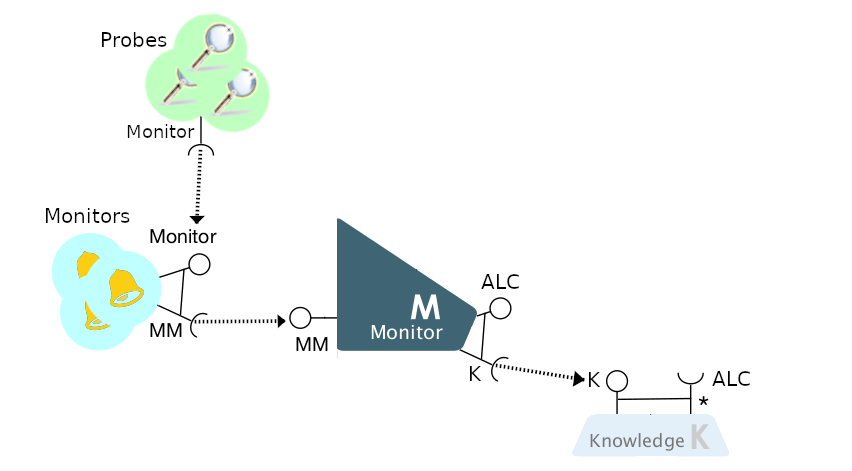
\includegraphics[scale=0.45]{cap_implementacion/images/hito-1-monitorizacion}
  \caption{Componentes desarrollados durante el primer hito: Sondas, monitores, el módulo de monitorización y el conocimiento.}
  \label{fig:hito-1-monitorizacion}
\end{figure}

\subsection{Peticiones síncronas}

En este hito se prototiparon las peticiones síncronas (flechas negras de la figura \ref{fig:hito-1-monitorizacion}). Los servicios que las implementan exponen APIs REST mediante \foreign{english}{endpoints} HTTP. Por ejemplo, el servicio de conocimiento expone operaciones que permiten recuperar o modificar propiedades de adaptación. Nos centraremos en la primera, ya descrita en la tabla \ref{tab:especificacion-get-property}.

En el fragmento \ref{ls:csharp-get} mostramos su implementación. Podemos observar que se trata de un método llamado \emph{GetProperty}. Su lógica es sencilla: busca en un diccionario la propiedad cuyo nombre recibe por parámetro. Si la encuentra, devuelve su valor con un código HTTP (\texttt{200 OK}). En caso contrario, sólo devuelve un código de error que describe el motivo de fallo: formato de la petición incorrecto (\texttt{400 - Bad Request}) o que no se ha encontrado la propiedad (\texttt{404 - Not Found}).

Podemos comprobar que el método cuenta con una serie de comentarios (líneas \texttt{1-8}) y atributos (\texttt{10-12}). En conjunto estos conforman su documentación. Describen qué hace el método, sus parámetros de entrada y posibles respuestas. OpenAPI puede aprovecharlos para generar una especificación más completa. Resulta entonces muy recomendable incluirlos.

\begin{lstlisting}[language={[Sharp]C},caption={Implementación del método \texttt{GetProperty} decorado para generar la especificación OpenAPI.\protect\footnotemark},captionpos=b, label=ls:csharp-get]
  /// <summary>
  ///    Gets a property given its name.
  /// </summary>
  /// <param name="propertyName"> The name of the property to find. </param>
  /// <returns> An IActionResult with result of the query. </returns>
  /// <response code="200"> The property was found. Returns the value of the property. </response>
  /// <response code="404"> The property was not found. </response>
  /// <response code="400"> There was an error with the provided arguments. </response>
  [HttpGet("{propertyName}")]
  [ProducesResponseType(typeof(PropertyDTO), StatusCodes.Status200OK)]
  [ProducesResponseType(StatusCodes.Status404NotFound)]
  [ProducesResponseType(StatusCodes.Status400BadRequest)]
  public IActionResult GetProperty([FromRoute]string propertyName)
  {
      if (string.IsNullOrEmpty(propertyName))
      {
          return BadRequest();
      }

      bool propertyFound =
          properties.TryGetValue(propertyName, out PropertyDTO property);

      if (!propertyFound)
      {
          return NotFound();
      }

      return Ok(property);
  }
\end{lstlisting}

\footnotetext{Código disponible \href{https://github.com/Starkie/TFM-DistributedAutoadaptiveSystems/blob/1db95346290cb55edbfd5efb717785bcd06def79/src/AutoAdaptativeSystem/AdaptionLoop/Knowledge/Controllers/PropertyController.cs\#L44-L77}{aquí}.}

Para generar la especificación empleamos la librería \emph{Swashbuckle.AspNetCore}\footnote{Página oficial: \url{https://github.com/domaindrivendev/Swashbuckle.AspNetCore}}. Esta es capaz de extraerla de un servicio ASP.NET existente. En el fragmento \ref{ls:openapi-get}, podemos ver cómo se describe el \foreign{english}{endpoint} en este estándar. Podemos confirmar que se han incluido los comentarios y atributos que documentaban en el código. Por ejemplo, figuran los parámetros, las respuestas y sus códigos HTTP, etc. Es destacable la similitud que presenta con la especificación de la tabla \ref{tab:especificacion-get-property}.

\begin{lstlisting}[language=python,caption={Especificación OpenAPI del método para obtener una propiedad del conocimiento (\lstinline{GetProperty}). \protect\footnotemark},captionpos=b, label=ls:openapi-get]
"paths": {
  "/Property/{propertyName}": {
    "get": {
      "tags": [
        "Property"
      ],
      "summary": "Gets a property given its name.",
      "parameters": [{
          "name": "propertyName",
          "in": "path",
          "description": "The name of the property to find.",
          "required": true,
          "schema": {
            "type": "string"
          }
        }
      ],
      "responses": {
        "200": {
          "description": "The property was found. Returns the value of the property.",
          "content": {
            "application/json": {
              "schema": {
                "$ref": "#/components/schemas/PropertyDTO"
              }
            }
          }
        },
        "404": { "description": "The property was not found.", },
        "400": {
          "description": "There was an error with the provided arguments.",
        }
      }
    }
  }
\end{lstlisting}

\footnotetext{Código disponible \href{https://github.com/Starkie/TFM-DistributedAutoadaptiveSystems/blob/1db95346290cb55edbfd5efb717785bcd06def79/src/AutoAdaptativeSystem/AdaptionLoop/Knowledge/Knowledge.Service-OpenAPISpec.json\#L108-L187}{aquí}.}

A partir de la especificación, esta librería añade a nuestro servicio una interfaz de usuario. Esta es accesible a través del \foreign{english}{endpoint} \texttt{/swagger}. Allí, se nos servirá una página web con el listado de todas las operaciones que ofrece el servicio (figura \ref{fig:swagger-knowledge-ui}). De cada una nos muestra su documentación, sus parámetros, etc. Incluso nos permite ejecutarlas. Así, puede ser de ayuda a los desarrolladores que necesiten trabajar con esta API.

\begin{figure}[htb]
  \centering
  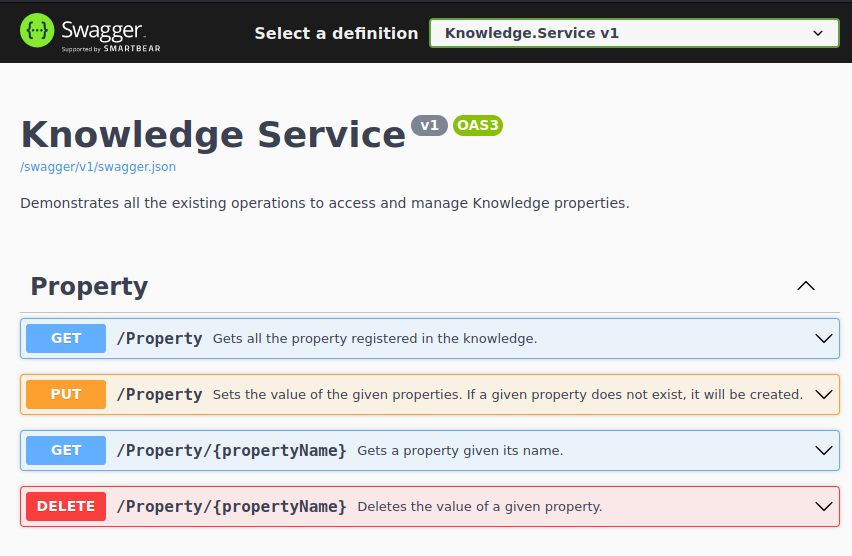
\includegraphics[scale=1.5]{cap_implementacion/images/swagger-knowledge-ui}
  \caption{Interfaz de usuario ofrecida por Swagger para el servicio de conocimiento. Se genera a partir de las especificación OpenAPI.}
  \label{fig:swagger-knowledge-ui}
\end{figure}

Por otro lado, también podemos generar el API \foreign{english}{client}. Como comentamos en la sección \ref{chap:OpenAPI} - \nameref{chap:OpenAPI}, tenemos gran variedad de generadores de código a nuestra disposición. Nosotros optamos por la librería \texttt{OpenAPI.Generator}\footnote{Página del proyecto: \url{https://github.com/OpenAPITools/openapi-generator}}. En concreto, por un generador de código de \verb|C#|. Usándolo, pudimos obtener una librería que permite contactar con nuestro servicio, sin necesidad de implementar mucho código. Por ejemplo, el componente de monitorización del bucle contacta con el conocimiento a través de un API \foreign{english}{client}.

Además, podremos utilizar estas herramientas durante la refactorización del bucle MAPE-K original. Aunque este está desarrollado en Java, podremos generar el código a partir de la especificación de nuestra implementación. Tanto de los clientes como los servidores. Esto ayudará a agilizar enormemente el proceso de desarrollo.

\subsection{Componentes: Módulos de monitorización y conocimiento}

Los componentes implementados en este hito son muy sencillos. Simplemente validan las mediciones de las sondas y extraen de ellas las propiedades de adaptación. Ya hemos hablado de la implementación del servicio de conocimiento. Este ofrece simplemente operaciones de lectura y escritura sobre las propiedades de adaptación y las claves de configuración de los recursos manejados.

Por encima de este, tenemos al servicio de monitorización. En nuestra implementación, actúa como intermediario entre los monitores de la solución y el conocimiento. Ofrece \foreign{english}{endpoints} útiles para los monitores, como puede ser reportar sus mediciones o la lectura del conocimiento. De esta forma, los monitores de solución podrán informarse para determinar si una medición es válida o no. Para conectar todos estos servicios se emplearon las peticiones síncronas, que describiremos anteriormente.

\section{Servicio de análisis y reglas}
\label{sec:implementacion-modulo-reglas}

La siguiente etapa que desarrollamos fue la evaluación de las reglas de adaptación. Esta requería implementar el servicio de análisis del bucle MAPE-K y los servicios de reglas de la solución. También necesitamos el mecanismo de las comunicaciones ascendentes: las notificaciones. Con ellas evitamos que los componentes se acoplaran a los de la capa superior.

\subsection{Notificaciones}

\begin{wrapfigure}{r}{0.13\linewidth}
  \vspace{-10pt}
  
\includegraphics[scale=0.09]{cap_implementacion/images/rabbitmq}
  \centering
  \vspace{-10pt}
\end{wrapfigure}

Comenzaremos describiendo el desarrollo de las notificaciones (flechas moradas de la figura \ref{fig:hito-2-analisis}). Como ya se describió en la sección \ref{sec:notificaciones}, este mecanismo se implementó mediante un \foreign{english}{broker} de mensajería. Elegimos \texttt{RabbitMQ}\footnote{Página oficial: \url{https://www.rabbitmq.com/}} para el proyecto, un \foreign{english}{broker} sencillo y ampliamente utilizado. \cite{newmanBuildingMicroservicesDesigning2021}

Para implementar los publicadores y consumidores de nuestro conector, utilizamos una librería llamada \texttt{Rebus}\footnote{Página oficial: \url{https://github.com/rebus-org/Rebus}}. Esta nos permitía interactuar con el bus abstrayéndonos de su tecnología concreta. Así, podríamos cambiar de tecnología de transporte en cualquier momento sin tener que modificar nuestros servicios.

Finalmente, para desacoplar la funcionalidad del servicio de la publicación y consumición de mensajes del bus, empleamos \texttt{MediatR}\footnote{Página oficial: \url{https://github.com/jbogard/MediatR}}. Esta librería implementa el patrón mediador\footnote{Patrón mediador: \url{https://refactoring.guru/design-patterns/mediator}}. Nos permite propagar mensajes dentro de un mismo proceso, sin necesidad de que el emisor ni el receptor se referencien. Para ello, se definen uno o más manejadores (\foreign{english}{handlers}) que capturan y procesan el mensaje. En el caso de las notificaciones propagaremos eventos de integración.

Para describir la implementación nos centraremos en la comunicación entre el módulo de conocimiento y el servicio de análisis. Una vez se confirma la escritura de una propiedad de adaptación en el conocimiento, este debe notificar a los servicios en la capa superior. Para ello, comienza propagando internamente un \textbf{evento de integración} usando el mediador (línea 11 del fragmento \ref{ls:knowledge-set-property}).

\begin{lstlisting}[language={[Sharp]C},caption={Implementación del método que asigna valor a una propiedad. Muestra un ejemplo de propagación interna de eventos de integración.\protect\footnotemark},captionpos=b, label=ls:knowledge-set-property]
private async Task SetProperty(SetPropertyDTO propertyDto)
{
    var newValue = new()
    {
        Value = propertyDto.Value,
        LastModification = DateTime.UtcNow,
    };

    properties.AddOrUpdate(propertyDto.Name, newValue, (_, _) => newValue);

    await _mediator.Send(
      new PropertyChangedIntegrationEvent(propertyDto.Name));
}

\end{lstlisting}

\footnotetext{Código disponible \href{https://github.com/Starkie/TFM-DistributedAutoadaptiveSystems/blob/1db95346290cb55edbfd5efb717785bcd06def79/src/AutoAdaptativeSystem/AdaptionLoop/Knowledge/Controllers/PropertyController.cs\#L106-L119}{aquí}.}

El mediador determina que el componente publicador es el destinatario de este evento y lo invoca. Para detectarlo, se basa en las interfaces que implementa (linea 2 del fragmento \ref{ls:knowledge-property-changed-publisher}). Este componente publica el evento en el bus de mensajería (línea 15). Rebus, en base a la configuración del servicio, lo enviará a nuestra instancia de \texttt{RabbitMQ}. Todos los suscriptores de este evento recibirán el mensaje en su cola.

\begin{lstlisting}[language={[Sharp]C},caption={El publicador de eventos captura el evento de integración y lo publica en el bus.\protect\footnotemark},captionpos=b, label=ls:knowledge-property-changed-publisher]
public class PropertyChangedIntegrationEventPublisher
  : IIntegrationEventPublisher<PropertyChangedIntegrationEvent>
{
  private readonly IBus _bus;

  public PropertyChangedIntegrationEventPublisher(IBus bus)
  {
      _bus = bus;
  }

  public async Task<Unit> Handle(
      PropertyChangedIntegrationEvent notification,
      CancellationToken cancellationToken)
  {
      await _bus.Publish(notification);

      return Unit.Value;
  }
}
\end{lstlisting}

\footnotetext{Código disponible \href{https://github.com/Starkie/TFM-DistributedAutoadaptiveSystems/blob/1db95346290cb55edbfd5efb717785bcd06def79/src/AutoAdaptativeSystem/AdaptionLoop/Knowledge/EventHandlers/PropertyChangedIntegrationEventPublisher.cs}{aquí}.}

Finalmente, en el servicio de análisis, tenemos el componente consumidor (fragmento \ref{ls:analysis-property-changed-consumer}). \texttt{Rebus} obtiene el evento de la cola de mensajería y se lo transmite. Este lo recibe y lo propaga internamente en el servicio (línea 20). Todos los \foreign{english}{handlers} del evento lo recibirán y podrán tratarlo. En este caso, las reglas de adaptación.

\begin{lstlisting}[language={[Sharp]C},caption={El consumidor recibe el evento de integración del bus y lo propaga internamente. Todos los \foreign{english}{handlers} de este evento lo recibirán.\protect\footnotemark},captionpos=b, label=ls:analysis-property-changed-consumer]
public class PropertyChangedIntegrationEventConsumer
  : IIntegrationEventConsumer<PropertyChangedIntegrationEvent>
{
  private readonly IMediator _mediator;

  public PropertyChangedIntegrationEventConsumer(IMediator mediator)
  {
      _mediator = mediator;
  }

  public async Task Handle(PropertyChangedIntegrationEvent message)
  {
      await _mediator.Publish(message);
  }
}
\end{lstlisting}

\footnotetext{Código disponible \href{https://github.com/Starkie/TFM-DistributedAutoadaptiveSystems/blob/1db95346290cb55edbfd5efb717785bcd06def79/src/AutoAdaptativeSystem/AdaptionLoop/Analysis/Application/Properties/Events/PropertyChangedIntegrationEventConsumer.cs}{aquí}.}

\subsection{Componentes: Servicio de análisis y módulos de reglas}

En este hito se desarrollaron los servicios de análisis y de los módulos de reglas (figura \ref{fig:hito-2-analisis}). En cuanto al del módulo de análisis, este realmente no cuenta con mucha lógica. Participa como intermediario entre el conocimiento y los servicios de reglas. Como hemos visto, recibe los eventos de cambios en las propiedades y los propaga a la capa superior. Ofrece operaciones de solo lectura del conocimiento. Así, impedimos las escrituras por parte de las reglas.

\begin{wrapfigure}{l}{0.3\linewidth}
  \vspace{-20pt}
  \centering
  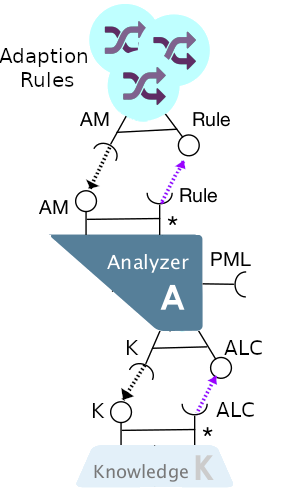
\includegraphics[scale=0.6]{cap_implementacion/images/hito-2-analisis}
\caption{Segundo hito: reglas de adaptación y módulo de análisis.}
  \label{fig:hito-2-analisis}
  \vspace{-10pt}
\end{wrapfigure}

Más tarde nos dimos cuenta que se podría considerar como un servicio ''anémico''\footnote{Similar a los objetos anémicos, sin apenas lógica: \url{https://www.martinfowler.com/bliki/AnemicDomainModel.html}}. \cite{singjaiPatternsDerivingAPIs2021} No tiene apenas lógica propia. Cuando se realice la refactorización del bucle original, se podría evalúar si tiene sentido mantener esta división. Si no es así, debería desplegarse como una librería que consuman todos los servicios de reglas de adaptación. En trabajos posteriores, este servicio podría ampliarse añadiendo autenticación y autorización. Así, se podría evitar que servicios no autorizados accedan a sus operaciones o soliciten adaptaciones maliciosas.

Respecto a los módulos de reglas, a continuación ofrecemos una implementación de referencia. En el fragmento \ref{ls:adaption-rule-base} mostramos la clase base de las reglas de adaptación. Se desarrolló siguiendo el patrón plantilla (o \foreign{english}{template})\footnote{\url{https://refactoring.guru/design-patterns/template-method}}. Define un método que evalúa la condición de la regla (\texttt{EvaluateCondition}) y, si esta se cumple, la ejecuta (\texttt{Execute}). Aquellas reglas que hereden de esta deberán de implementar ambos métodos.

Vemos además que está suscrita a los eventos de integración de cambio de propiedad de adaptación y cambio en la configuración del sistema (lineas 2-3). Cuando el consumidor reciba uno de ellos, lo propagará internamente. Todas las reglas afectadas lo capturarán y se evaluarán.

\begin{lstlisting}[language={[Sharp]C},caption={Clase base para implementar reglas de adaptación. Se evalúa la condición, y si esta se cumple, se ejecuta. \protect\footnotemark},captionpos=b, label=ls:adaption-rule-base]
public abstract class AdaptionRuleBase
    : IIntegrationEventHandler<PropertyChangedIntegrationEvent>,
      IIntegrationEventHandler<ConfigurationChangedIntegrationEvent>
{
    // ..
    private async Task Handle()
    {
        try
        {
            if (await EvaluateCondition())
            {
                await Execute();
            }
        }
        catch (Exception e)
        {
            _diagnostics.RuleEvaluationError(_ruleName, e);

            throw;
        }
    }

    protected abstract Task<bool> EvaluateCondition();

    protected abstract Task Execute();
}
\end{lstlisting}

\footnotetext{Código disponible \href{https://github.com/Starkie/TFM-DistributedAutoadaptiveSystems/blob/1db95346290cb55edbfd5efb717785bcd06def79/src/AutoAdaptativeSystem/Climatisation/Rules/EventHandlers/Rules/AdaptionRuleBase.cs}{aquí}.}

Las reglas deben indicar de qué propiedades o claves de configuración dependen. Para ello, hemos implementado una serie de atributos que decoran sus clases. En el fragmento \ref{ls:adaption-rule-dependencies} mostramos un ejemplo. En la línea 1 tenemos el atributo que describe las dependencias con la propiedad de adaptación \texttt{Temperature}. Por otro lado, en las líneas 2-5 tenemos la declaración de dependencias con dos claves de configuración del servicio \texttt{Climatisation.AirConditioner}: \texttt{TargetTemperature} y \texttt{Mode}.

\begin{lstlisting}[language={[Sharp]C},caption={Las reglas declaran sus dependencias sobre propiedades de adaptación usando atributos. Estos se utilizarán para las suscripciones a los temas de los eventos.\protect\footnotemark},captionpos=b, label=ls:adaption-rule-dependencies]
[RuleKnowledgePropertyDependency(ClimatisationConstants.Property.Temperature)]
[RuleServiceConfigurationDependency(
    ClimatisationAirConditionerConstants.AppName,
    ClimatisationAirConditionerConstants.Configuration.TargetTemperature,
    ClimatisationAirConditionerConstants.Configuration.Mode)]
public class DisableAirConditionerWhenCoolingAndTargetTemperatureAchievedAdaptionRule
  : AdaptionRuleBase
{
    // ...
}
\end{lstlisting}

\footnotetext{Código disponible \href{https://github.com/Starkie/TFM-DistributedAutoadaptiveSystems/blob/1db95346290cb55edbfd5efb717785bcd06def79/src/AutoAdaptativeSystem/Climatisation/Rules/EventHandlers/Rules/DisableAirConditionerWhenCoolingModeEnabledAndTargetTemperatureAchievedRule.cs\#L14-L19}{aquí}.}

En base a los atributos, el servicio se suscribirá a los \foreign{english}{topics} de las notificaciones que emite el módulo de análisis. Para leerlos emplearemos la \textbf{reflexión}: analizaremos el ensamblado buscando las reglas y obtendremos los valores de sus atributos. Se le pasarán a \texttt{Rebus}, que gestionará la suscripción con \texttt{RabbitMQ}.

\section{Servicio de planificación y peticiones de cambio}

En el tercer hito implementamos las peticiones de cambio en la configuración del sistema. Este proceso comienza con la ejecución del cuerpo de las reglas y acaba con la generación de un \textbf{plan de cambio}. Esto requirió del desarrollo de un nuevo servicio: el planificador (figura \ref{fig:hito-3-planificador}). En este hito también surgió la necesidad de las peticiones asíncronas, el tercer protocolo de comunicación.

\begin{figure}[h!]
  \centering
  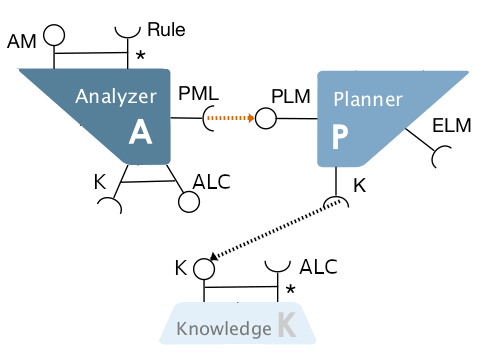
\includegraphics[scale=0.50]{cap_implementacion/images/hito-3-planificador}
  \caption{Componente desarrollado durante el tercer hito: Planificador.}
  \label{fig:hito-3-planificador}
\end{figure}

\subsection{Peticiones asíncronas}

Las peticiones asíncronas son el tercer mecanismo de comunicación de nuestra arquitectura (flecha naranja en la figura \ref{fig:hito-3-planificador}). Estas permiten interactuar a los servicios que pertenecen a una misma capa. Para describir su implementación tomaremos de ejemplo las peticiones de cambio de las reglas de adaptación.

Cuando la regla evalúa su condición y estima que es necesaria una acción correctiva, se ejecuta su método \texttt{Execute}. Este método envía una petición que describe cuál debería ser el siguiente estado del recurso manejado. Por ejemplo, qué componentes deben estar presentes o no, qué conexiones deben existir, etc.

Las reglas comunicarán esta solicitud al módulo de análisis mediante una petición síncrona. Para simplificar el proceso, desarrollamos un \foreign{english}{builder}\footnote{Patrón \foreign{english}{builder}: \url{https://refactoring.guru/design-patterns/builder}} de peticiones por encima de su API \foreign{english}{client}. En el fragmento \ref{ls:change-request-builder} mostramos un ejemplo. Allí se indica cuál debería ser la siguiente configuración para el servicio \texttt{Climatisation AirConditioner Service} (líneas 7-14). Deberá estar activo (línea 10) y su propiedad \texttt{Mode} deberá tener el valor \texttt{Cooling} (líneas 11-13). También se incluye el síntoma que desencadena el cambio (línea 6).

\begin{lstlisting}[language={[Sharp]C},caption={Implementación de la misma petición siguiendo el patrón \emph{builder}.\protect\footnotemark},captionpos=b, label=ls:change-request-builder]
protected override async Task Execute()
{
  await _systemService.RequestConfigurationChange(changeRequest =>
  {
    changeRequest
      .ForSymptom(TemperatureGreaterThanHotThreshold)
      .WithService(ClimatisationAirConditionerConstants.AppName, service =>
      {
        service
          .MustBePresent()
          .WithParameter(
            ClimatisationAirConditionerConstants.Configuration.Mode,
            AirConditioningMode.Cooling.ToString());
      });
  });
}
\end{lstlisting}

\footnotetext{Código disponible \href{https://github.com/Starkie/TFM-DistributedAutoadaptiveSystems/blob/1db95346290cb55edbfd5efb717785bcd06def79/src/AutoAdaptativeSystem/Climatisation/Rules/EventHandlers/Rules/DisableAirConditionerWhenCoolingModeEnabledAndTargetTemperatureAchievedRule.cs\#L74-L88}{aquí}.}

El servicio de análisis recibirá la petición y la redirigirá al planificador mediante una petición asíncrona. Su implementación es muy similar a la de las notificaciones, explicada en detalle en el apartado anterior. La mayor diferencia radica en la cardinalidad de la comunicación: en lugar de publicarlo en un \foreign{english}{exchange}, el mensaje se publicará directamente en la cola de trabajo. Sólo lo debería procesará un servicio.

Como la comunicación es tan similar, únicamente cambiará la implementación del publicador. La mayor diferencia la podemos apreciar en el fragmento \ref{ls:request-publisher}. Allí, vemos que el mensaje se enruta directamente a la cola \texttt{PlanningServiceQueue} (línea 15). También cambiarán las interfaces que deban implementar los componentes. En este caso \texttt{IRequestPublisher} en lugar de \texttt{IIntegrationEventPublisher} (línea 2).

\begin{lstlisting}[language={[Sharp]C},caption={Las peticiones asíncronas se publican a una cola determinada.\protect\footnotemark},captionpos=b, label=ls:request-publisher]
public class SystemConfigurationChangeRequestPublisher
  : IRequestPublisher<SystemConfigurationChangeRequest>
  where TRequest : Request
{
  public SystemConfigurationChangeRequestPublisher(IBus bus)
  {
      _bus = bus;
  }

  public async Task<Unit> Handle(
      SystemConfigurationChangeRequest request,
      CancellationToken cancellationToken)
  {
      await _bus.Advanced.Routing.Send(
          AdaptionLoopPlanningConstants.Queues.PlanningServiceQueue,
          request);

      return Unit.Value;
  }
}
\end{lstlisting}

\footnotetext{Código disponible \href{https://github.com/Starkie/TFM-DistributedAutoadaptiveSystems/blob/1db95346290cb55edbfd5efb717785bcd06def79/src/AutoAdaptativeSystem/AdaptionLoop/Analysis/Application/SystemConfiguration/Requests/SystemConfigurationChangeRequestIntegrationEventPublisher.cs}{aquí}.}


\subsection{Componentes: Servicio de planificación}

El planificador consumirá esta petición de cambio y deberá elaborar un \textbf{plan de adaptación}. Para ello, deberá determinar qué acciones son necesarias para alcanzar el estado deseado. Lo comparará con el estado actual, almacenado en el conocimiento, y añadirá al plan las \textbf{acciones de adaptación} requeridas. Si el sistema ya estuviera en ese estado, el plan de cambio se quedará vacío y no se propagará.

Por ejemplo, en el fragmento \ref{ls:adaption-change-plan} encontramos un plan de adaptación para la regla descrita en la sección anterior. Solo contiene una acción de adaptación: cambiar el valor de la propiedad \texttt{Mode} a \texttt{Cooling}. Como el servicio de aire acondicionado ya estaba en funcionamiento, no se ha incluido una acción para desplegarlo.

\begin{lstlisting}[language=python,caption={Plan de adaptación generado para la regla anterior. Solo contiene una acción de adaptación: cambiar la configuración \texttt{Mode} del servicio \texttt{AirConditioner}.},captionpos=b, label=ls:adaption-change-plan]
{
  "ChangePlan": {
    "Timestamp": "2022-07-09T09:53:01.1868834Z",
    "Actions":
    [
      {
        "Type": "SetParameter",
        "ServiceName": "Climatisation.AirConditioner.Service",
        "PropertyName": "Mode",
        "PropertyValue": "Cooling"
      }
    ]
  },
  "Symptoms":
  [
    {
      "Name": "temperature-lesser-than-cold-threshold",
      "Value": "true"
    }
  ]
}
\end{lstlisting}

Para reducir el alcance del proyecto, no validaremos la viabilidad del plan de adaptación. Se descartó implementar los planificadores específicos de la solución.  Sólo contaremos con la estrategia por defecto: validar que el plan contenga al menos un acción.


\section{Servicio de ejecución y efectores}


En el hito final desarrollamos la ejecución del plan de adaptación. Cerramos así el ciclo del bucle de adaptación. Esto requirió del módulo ejecutor, los ejecutores de la solución y los efectores del recurso manejado (figura \ref{fig:hito-4-ejecutor}).

\begin{figure}[h!]
  \centering
  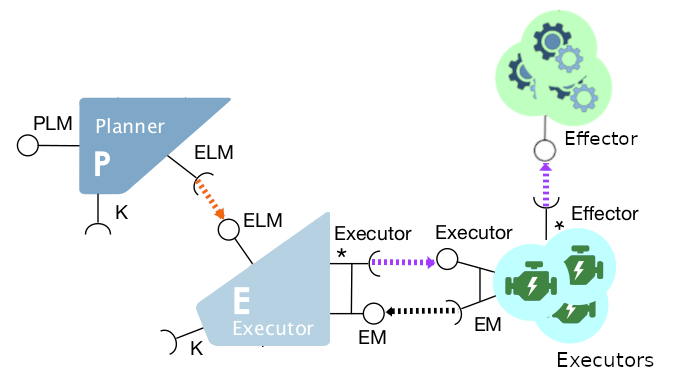
\includegraphics[scale=0.55]{cap_implementacion/images/hito-4-ejecutor}
  \caption{Componentes desarrollados durante el cuarto hito: Módulo de ejecución, ejecutores y efectores.}
  \label{fig:hito-4-ejecutor}
\end{figure}

\subsection{Componentes: Servicio de ejecución, ejecutores y efectores}

El servicio de ejecución recibe el plan de adaptación del planificador mediante una petición asíncrona. Para ejecutarlo, deberá agrupar las acciones por el servicio afectado y distribuirlas entre los distintos ejecutores de la solución. Para transmitirlas, enviará cada grupo de acciones mediante una notificación. Pueden existir varios ejecutores de la solución, y no deberíamos acoplarnos a ellos. El evento enviado es muy similar al que ya mostramos en el fragmento \ref{ls:adaption-change-plan}.

Cuando un ejecutor capture esta notificación, procesará las acciones asignadas. Este componente será el encargado de traducir las acciones de adaptación a manipulaciones de efectores del recurso manejado. Dependiendo del tipo de acción, el efector hará una acción u otra: desplegar un servicio, o eliminarlo, cambiar la configuración, etc. Para reducir el alcance del proyecto, sólo implementamos las adaptaciones de tipo \foreign{english}{set parameter}.

En cuanto a la comunicación con el efector, este caso es un tanto especial. El mecanismo dependerá del sistema manejado; de si tenemos control sobre su implementación. Si no es así, tendremos que adaptarnos a aquellos protocolos que ofrezca el recurso (HTTP, mensajería...).

Continuando con el ejemplo del aire acondicionado, el ejecutor recibiría la notificación con las acciones a ejecutar. En este caso, cambiar el modo de funcionamiento a enfriar. Para ello, enviará la acción al efector y se ejecutará. Una vez se confirme el cambio, una sonda lo detectará y notificará a su monitor. Se seguirá el mismo proceso que con las demás mediciones para guardarlo en la base de conocimiento.
